\documentclass[12pt]{article}
\usepackage[utf8]{inputenc}
\usepackage[spanish,es-lcroman, es-tabla]{babel}
\usepackage[autostyle,spanish=mexican]{csquotes}
\usepackage{amsmath}
\usepackage{amssymb}
\usepackage{nccmath}
\numberwithin{equation}{section}
\usepackage{amsthm}
\usepackage{graphicx}
\usepackage{epstopdf}
\DeclareGraphicsExtensions{.pdf,.png,.jpg,.eps}
\usepackage{color}
\usepackage{float}
\usepackage{multicol}
\usepackage{enumerate}
\usepackage[shortlabels]{enumitem}
\usepackage{anyfontsize}
\usepackage{anysize}
\usepackage{array}
\usepackage{multirow}
\usepackage{enumitem}
\usepackage{cancel}
\usepackage{tikz}
\usepackage{circuitikz}
\usepackage{tikz-3dplot}
\usetikzlibrary{babel}
\usetikzlibrary{shapes}
\usepackage{bm}
\usepackage{mathtools}
\usepackage{esvect}
\usepackage{hyperref}
\usepackage{relsize}
\usepackage{siunitx}
\usepackage{physics}
%\usepackage{biblatex}
\usepackage{standalone}
\usepackage{mathrsfs}
\usepackage{bigints}
\usepackage{bookmark}
\spanishdecimal{.}

\setlist[enumerate]{itemsep=0mm}

\renewcommand{\baselinestretch}{1.5}

\let\oldbibliography\thebibliography

\renewcommand{\thebibliography}[1]{\oldbibliography{#1}

\setlength{\itemsep}{0pt}}
%\marginsize{1.5cm}{1.5cm}{2cm}{2cm}


\newtheorem{defi}{{\it Definición}}[section]
\newtheorem{teo}{{\it Teorema}}[section]
\newtheorem{ejemplo}{{\it Ejemplo}}[section]
\newtheorem{propiedad}{{\it Propiedad}}[section]
\newtheorem{lema}{{\it Lema}}[section]

\title{Cadena colgante que oscila \\ {\large Tema 5 - Matemáticas Avanzadas de la Física}\vspace{-1.5\baselineskip}}
\date{ }
\author{}
\begin{document}
\maketitle
\fontsize{14}{14}\selectfont
\section*{Introducción}
Uno de los problemas clásicos de la teoría de las oscilaciones se refiere a las pequeñas oscilaciones de una cadena colgante flexible. Este problema fue discutido por primera vez en 1732 por D. Bernoulli y más tarde en 1781 por Euler, para ambos casos, años antes del legendario documento de Bessel en 1824 sobre las propiedades de las funciones de Bessel.
\section{Desarrollo.}
\begin{wrapfigure}{L}{0.4\textwidth}
    \centering
    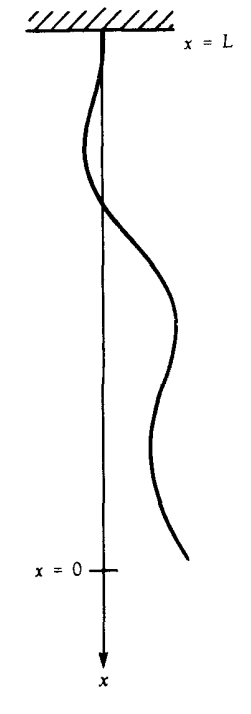
\includegraphics[scale=0.25]{Imagenes/Cadena_Oscilante.png}
    \caption{Cadena colgante que está oscilando.}
    \label{fig:figura_cadena_01}
\end{wrapfigure}

Considera una cadena pesada y flexible de longitud $L$, fija en el extremo superior y libre en el extremo inferior (ver Fig. \ref{fig:figura_cadena_01}). Cuando la cadena se perturba ligeramente desde su posición de equilibrio en un plano vertical, experimenta oscilaciones \enquote{pequeñas}. Sea $\rho$ la densidad de masa constante por unidad de longitud, sea $y$ el desplazamiento horizontal de la cadena en el tiempo $t$. Tomando el origen en la parte inferior de la cadena como se muestra en la Fig. (\ref{fig:figura_cadena_01}), la fuerza resultante por unidad de longitud $x$ es
\begin{align*}
\pdv{x} \left( T \, \pdv{y}{x} \right)
\end{align*}
donde $T$ es la tensión en la cadena. Igualando esta fuerza resultante a
\begin{align*}
\rho \pdv[2]{y}{t}
\end{align*}
que representa el producto de la masa (por unidad de longitud) y la aceleración, obtenemos la ecuación de movimiento, es decir, la segunda ley de Newton
\begin{equation}
\pdv{x} \left( T \, \pdv{y}{x} \right) = \rho \pdv[2]{y}{t}
\label{eq:ecuacion_06_106}
\end{equation}
Supongamos que la tensión $T$ se debe enteramente al peso de la cadena debajo de un punto $x$ determinado. En este caso, $T = \rho \, g \, x$, donde $g$ es la constante gravitacional, y la ec. (\ref{eq:ecuacion_06_106}) toma la forma
\begin{equation}
g \, \pdv{x} \left( x \, \pdv{y}{x} \right) = \pdv[2]{y}{t}
\label{eq:ecuacion_06_107}
\end{equation}
Dado que la cadena está fija en la parte superior, donde $x = L$ y está libre en la parte inferior donde $x = 0$, las CDF que la acompañan están dadas por
\begin{equation}
\abs{y(0)} < \infty \hspace{2cm} y(L) = 0
\label{eq:ecuacion_06_108}
\end{equation}
La primera condición simplemente requiere que el desplazamiento permanezca acotado en $x = 0$.
\par
Si bien la ec. (\ref{eq:ecuacion_06_107}) es una EDP, podemos reducirla a una EDO al suponer la variación de $y$ con respecto al tiempo $t$. Es decir, si asumimos que las oscilaciones $y$ son esencialmente sinusoidales con la frecuencia (angular) $\omega$, entonces podemos encontrar los \emph{modos normales de vibración} haciendo la sustitución
\begin{equation}
y =  R \, \cos (\omega \, t - \phi)
\label{eq:ecuacion_06_109}
\end{equation}
en la ec. (\ref{eq:ecuacion_06_107}), donde la amplitud $R$ es una función de $x$ nada más, y $\phi$ es un ángulo de fase. Luego de hacer esto, y dividir la ecuación resultante por $\cos (\omega \, t - \phi)$, obtenemos una EDO
\begin{equation}
x \, R^{\prime \prime} + R^{\prime} + k^{2} \, R = 0, \hspace{2cm} k^{2} = \dfrac{\omega^{2}}{g}
\label{eq:ecuacion_06_110}
\end{equation}
Reconocemos en la ec. (\ref{eq:ecuacion_06_110}) la expresión
\begin{equation}
x^{2} \, y^{\prime \prime} + (1 - 2 \, a) x \, y^{\prime} + [b^{2} \, c^{2} \, x^{2c} + (a^{2} - c^{2} \, p^{2}) ] \, y = 0, \hspace{1cm} p \geq 0, \hspace{0.5cm} b > 0
\label{eq:ecuacion_06_098}
\end{equation}
que tiene por solución
\begin{equation}
y = x^{a} [C_{1} \, J_{p} (b \, x^{c}) + C_{2} \, Y_{p} (b \, x^{c})]
\label{eq:ecuacion_06_099}
\end{equation}
Entonces para la ec. (\ref{eq:ecuacion_06_110}) se tiene que $a = 0$, $b = 2 \, k$, $c = 1/2$ y $p=0$. Por lo que la solución general está dada por
\begin{equation}
R(x) = C_{1} \, J_{0} (2 \, k \, \sqrt{x}) + C_{2} \, Y_{0} (2 \, k \, \sqrt{x})]
\label{eq:ecuacion_06_111}
\end{equation}
donde $C_{1}$ y $C_{2}$ son constantes arbitrarias.
\par
Para satisfacer la condición en $x = 0$, entonces debe ocurrir que $C_{2} = 0$, ya que $Y_{0}$ no está acotada para argumentos pequeños. La otra condición en $x = L$, nos lleva a
\begin{equation}
J_{0} (2 \, k \sqrt{L}) = 0
\label{eq:ecuacion_06_112}
\end{equation}
Para satisfacer ésta última relación, debemos de elegir los valores de $k$, $k_{1}, k_{2}, k_{3}, \ldots, k_{n}$, tales que $2 \, k \sqrt{L}$ siempre correspondan a una raíz de $J_{0}$. Estos valores de $k$ determinan a su vez las frecuencias de vibración permitidas a través de la relación
\begin{equation}
\omega_{n} = k_{n} \sqrt{g} \hspace{1.5cm} n = 1, 2, 3, \ldots
\label{eq:ecuacion_06_113}
\end{equation}
Por lo tanto, los correspondients modos normales de vibración son de la forma
\begin{equation}
y_{n} (x, t) = A_{n} \, J_{0} (2 \, k_{n} \sqrt{x}) \, \cos (\omega_{n} \, t - \phi_{n}) \hspace{1.5cm} n = 1, 2, 3, \ldots
\label{eq:ecuacion_06_114}
\end{equation}
donde $A_{n}$ y $\phi_{n}$ son constantes arbitrarias.



%La descripción de las oscilaciones de una cadena colgante fue un problema en la mecánica resuelta por Daniel Bernoulli en el siglo XVIII y que llevó al descubrimiento de la clase de funciones conocidas como funciones de Bessel.

%Se considera que la cadena es un cuerpo estrecho y continuo de longitud $L$, con una densidad de masa lineal $\mu$, suspendida desde un punto fijo. Fijando el origen del sistema de referencia en el extremo libre de la cadena, en su configuración de equilibrio (¡colgando verticalmente hacia abajo!), y el eje $z$ que apunta hacia arriba; los desplazamientos de la cadena se producen en el plano $xz$ (la cadena está fija en el punto $(0, L)$), y suponemos que los desplazamientos desde el punto de equilibrio son pequeños, por lo que no es necesario distinguir entre las distancias medidas a lo largo de la cadena y las distancias a lo largo de $z$.

% Con tales pequeños desplazamientos, la tensión en la cadena actúa principalmente en la dirección vertical: $T (z) = \mu \, g \, z$. Cualquier fuerza neta transversal en un elemento de masa infinitesimal doblada a través de un ángulo $\alpha$ se debe a la diferencia en la componente $x$ de la tensión por encima y por debajo de ella:
% \begin{align*}
% \dd{T_{z}} = \dd{(\mu \, g \, z \, \sin \alpha)} \simeq \dd{(\mu \, g \, z \, \tan \alpha)} = \dd{\left( \mu \, g \, z \, \dv{x}{z} \right)}
% \end{align*}
\end{document}